\section{Particle Size Determination}

Particle Size determination Info Here

From Paper:

Once the retrieval has been preformed for a complete series of wavelengths; determination of the Angstr\"{o}m exponent occurs which is preformed in a similar manor as outlined by \cite{Rault2013} for the OMPS aerosol particle size retrieval. The Angstr\"{o}m exponent is an approximation to Mie scattering since the value of the Angstr\"{o}m exponent, $\alpha$, is an analogy to particle size. Lower Angstr\"{o}m exponents correspond to larger particle sizes and vice versa for small particle sizes. Since the measurements observe relatively the same atmosphere over the time of one complete aerosol cycle; the differences between extinction ratios at the different wavelength can be used to gather a understanding of aerosol particle size in the form
\begin{equation}
    \frac{n\sigma}{n_{0}\sigma_{0}} = \left(\frac{\lambda}{\lambda_{0}}\right)^{-\alpha}
    \label{eqn:agstromCoefficient}
\end{equation}
where $n$ is the aerosol concentration, and $\sigma$ is the scattering cross section. Since the cross section of aerosol is dependent on not only the wavelength but also the particle size and distribution the Angstr\"{o}m exponent gives some information on particle size distribution. For the retrieval described here a single mode log-normal distribution is assumed with a mode radius, $r_{g}$, and the mode width, $\sigma_{g}$, which is the same as the OSIRIS version 5.07 aerosol product. At each retrieved altitude the extinction from each wavelength is used to fit the Angstr\"{o}m exponent. Then the median value from all the retrieved altitudes is used as the new size parameters in next iteration of the retrieval. The mode width is set at a constant 1.6 and the mode radius is allowed to vary to match the Angstr\"{o}m exponent retrieved. The mode radius is updated and the process is repeated, re-retrieving the extinction profiles, until the Angstr\"{o}m exponent converges. At the end of the last iteration, the Angstr\"{o}m exponent profile is reported as the final particle size product.

Results:

The particle size method was used as outlined in the pervious section. An Angstr\"{o}m exponent was retrieved for one instance of the ALI mission. The first panel of \autoref{fig:ParticleSize} shows the median Angstr\"{o}m exponent that was determined after each iteration and convergence can be seen after a couple iterations. The particle size determined for ALI in the last complete set of aerosol images can be seen in the second panel of \autoref{fig:ParticleSize} which yields a final Angstr\"{o}m exponent of between 2 and 3 throughout the altitude range from 13 to 25~km. Assuming a mode width of 1.6 yields a median mode radius of 0.083~\si{\micro\metre}.

In order to determine the Angstr\"{o}m exponent a least squares fit was used for all usable wavelengths at each altitude. A wavelength at a altitude was rejected if the forward model at that shell altitude was not within 3\% of the measurement vector. In the case shown in \autoref{fig:ParticleSize}, the 20.5~km shell altitude, only 11 of the 13 possible wavelengths contributed to the determination of the Angstr\"{o}m exponent.

\begin{figure}
\centering
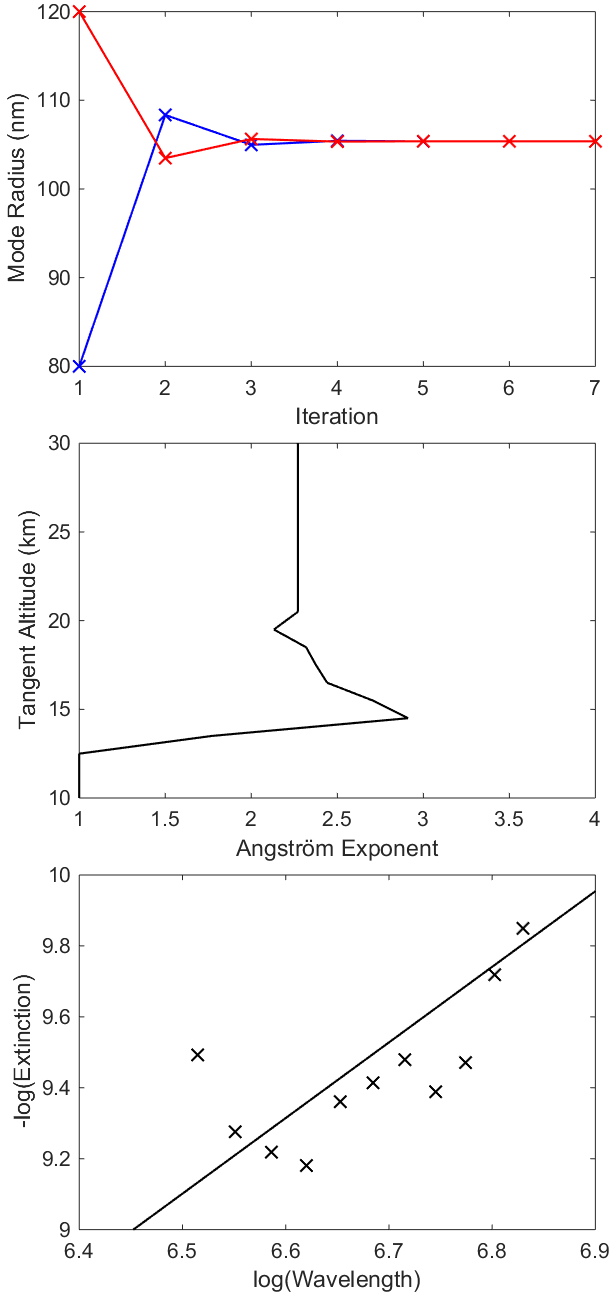
\includegraphics[width=0.5\textwidth]{./Images/5-4-ParticleSize.pdf}
    \caption[TODO:Write This]{The top panel shows the convergence of the mode radius throughout the iterations in the retrieval. The second panel is the final Angstr\"{o}m exponents determined for images 204-217 during the Timmins 2014 campaign. And the last panel demonstrate a least squares fit to determine the Angstr\"{o}m exponent at 20.5~km shell altitude.}
    \label{fig:5.4:ParticleSize}
\end{figure} 